\documentclass[
12pt,
a4paper,
bibliography=totocnumbered, %Literaturverzereichnis als Eintrag ins Inhaltsverzeichnis
%twoside, %Zweiseitiger Druck
BCOR=1cm, %Platz zum Lochen
oneside, %Einseitiger Druck
]{scrartcl}

\usepackage{geometry}

\usepackage[default]{fontsetup}
%\usepackage[onehalfspacing]{setspace}

\usepackage[ngerman]{babel}
\usepackage[babel=true,german=quotes]{csquotes}

\usepackage{microtype}
\usepackage{mleftright}
%\newcommand{\Le}{\mleft}
%\newcommand{\Ri}{\mright}
\usepackage[no-script, no-scriptscript, no-inner, no-close]{innerscript}

% Mathepakete (unicode-math ersetzt amssymb, amsfonts etc.)
\usepackage{amsmath,amsthm}
\usepackage{mathtools}
\usepackage{fixdif,derivative}
\usepackage{physics2}
\usephysicsmodule{ab.legacy}

\usepackage{unicode-math}
\setmathfont{NewCMMath-Book}
\setmathfont{NewCMMath-Book}[range=cal, StylisticSet=1]
\setmathfont{NewCMMath-Book}[range=scr]

\usepackage{siunitx}
\sisetup{detect-weight=true, detect-family=true,locale=DE,range-phrase={\,bis\,},list-final-separator ={\,\linebreak[0] \text{und}\,},separate-uncertainty=true,per-mode = symbol-or-fraction}
%\SI[per-mode = fraction]{1}{\meter\per\second} erzwingt auch im Fließtext die Bruchdarstellung.
\DeclareSIUnit\curie{Ci}%Zusätzliche Einheit definieren

\usepackage{tabularx, booktabs, multirow}
\usepackage{array}
\usepackage{enumitem}
\usepackage{float}
\usepackage{graphicx}
\usepackage{xurl}

\usepackage[final]{pdfpages}
\usepackage{framed, color} %Framed: Paket, mittels dessen ein Rahmen um einen Bereich definiert werden kann. Color: Lässt Farbdarstellung in Schrift, Hintergrund etc. zu

\usepackage{scrlayer-scrpage} %Header für die KOMA-script-Klasse

%\usepackage[square,numbers]{natbib}
\usepackage{subfigure} %Mehrere Bilder in einer Figure-Umgebung

\usepackage[bookmarks,colorlinks=true]{hyperref}
\hypersetup{
	colorlinks,
	linktocpage,
	citecolor=black,
	filecolor=black,
	linkcolor=black,
	urlcolor=black,
	pdftitle=X,
	pdfauthor=JM-VS
}

\usepackage[backend=biber, style=chem-angew]{biblatex}
\addbibresource{lit.bib}

\numberwithin{equation}{section} % Die Nummerierung von Gleichungen bekommt die jeweilige Section-Nummer als Präfix

\setlength{\parindent}{0pt} %Einrücktiefe von neuen Absätzen
\setlength{\parskip}{6pt} %Abstand von Absätzen

\pagestyle{scrheadings}%Kopf und Fußzeilen
\ohead{\textbf{\GRUPPENNR\ - \VERSUCHSNR}} %Header oben links auf linker Seite (ungerade Seitenzahl) und oben rechts auf rechter Seite (gerade Seitenzahl), beinhaltet gruppennummer und Versuchskürzel. Im Fall eine einseitigen Dokuments: Header oben rechts
\ihead{\VerfasserEINS\;\&\;\VerfasserZWEI} %Header oben rechts auf linker Seite und oben links auf rechter Seite. Beinhaltet die Namen der Verfasser. Im Fall eine einseitigen Dokuments: Header oben links!
\ofoot{\thepage} %Footer unten links auf linker und unten rechts auf rechter Seite, enthält die jeweilige Seitenzahl. Im Fall eines einseitigen Elements: Footer unten rechts!
\cfoot{\empty} %Mittig unten im Footer soll nichts eingetragen werden
\ifoot{\empty} %Footer unten rechts auf linker und unten links auf rechter Seite. Hier ebenfalls leer.

\newcommand{\tz}{T_{\text{II}}}
\newcommand{\ts}{T_{\text{S}}}
\newcommand{\tgl}{T_{\text{gl}}}
\newcommand{\tgeg}{T_{\text{geg}}}
\newcommand{\omz}{\omega_{\text{II}}}
\newcommand{\omgl}{\omega_{\text{gl}}}
\newcommand{\omgeg}{\omega_{\text{geg}}}
\newcommand{\kB}{k_{\text{B}}}

% Hier können die individuellen Anpassungen vorgenommen werden, die sich auf das Titelblatt und die Kopfzeilen auswirken.

\newcommand{\VERSUCHSDATUM}{29.09.2025}
\newcommand{\PROTOKOLLDATUM}{\today}

\newcommand{\VerfasserEINS}{Julian Molt}
\newcommand{\MatNoEINS}{3803097}
\newcommand{\StudiengangEINS}{Physik}

\newcommand{\VerfasserZWEI}{Valentin Stopper}
\newcommand{\MatNoZWEI}{3774391}
\newcommand{\StudiengangZWEI}{Physik}

\newcommand{\BETREUER}{Julian Vollmer}
\newcommand{\GRUPPENNR}{A-016}

\newcommand{\VERSUCHSNR}{E24}
\newcommand{\VERSUCHSNAME}{Halbleiterdioden}

\newcommand{\lh}{\ell_{\mathrm{H}}}
\newcommand{\ls}{\ell_{\mathrm{S}}}


\begin{document}

\thispagestyle{empty}

\begin{titlepage}

	\begin{center}
		\Huge{\textbf{\VERSUCHSNR\ -- \VERSUCHSNAME}}\\
		\vspace{10mm}
		\Large{Protokoll zum Versuch des Physikalischen Praktikums I von \\ \textbf{\VerfasserEINS\;\& \VerfasserZWEI}}\\
		\vspace{10mm}
		\Large{Universität Stuttgart}\\
	\end{center}
	\vspace{1cm}
	\begin{center}
		\begin{tabular}{ll}
			\large{Verfasser:}		& \large{\VerfasserEINS\;(\StudiengangEINS),} \\
			& \large{\MatNoEINS} \\
			\vspace{0cm}\\
			& \large{\VerfasserZWEI\;(\StudiengangZWEI),} \\
			& \large{\MatNoZWEI} \\
			\vspace{0cm}\\
			\large{Gruppennummer:}	& \large{\GRUPPENNR} \\
			\vspace{0cm}\\
			\large{Versuchsdatum:}	& \large{\VERSUCHSDATUM} \\
			\vspace{0cm}\\
			\large{Betreuerin:}		& \large{\BETREUER}
		\end{tabular}
	\end{center}
	\vspace{15mm}

	\begin{center}
		Stuttgart, den \PROTOKOLLDATUM
	\end{center}

\end{titlepage}

\thispagestyle{empty}

\tableofcontents

\clearpage %Neue Seite, davor werden alle noch ausstehenden Grafiken/Tabellen platziert.

\renewcommand{\thepage}{\arabic{page}}
\setcounter{page}{1}


% Die erste eckige Klammer ist optional, die darin angegebene Bezeichnung steht im Inhaltsverzeichnis anstelle des hinteren (längeren) Namens.
\section[Versuchsziel]{Versuchsziel und Versuchsmethode}

In diesem Versuch werden Halbleiterdioden untersucht. Dazu werden die Kennlinien einer Silizium- und Germaniumdiode, einer Z-Diode und von zwei LEDs aufgezeichnet. Für die Z-Diode und die LEDs geschieht dies mithilfe eines Oszilloskops.

\section{Grundlagen}


%\begin{figure}[H]
%	\centering{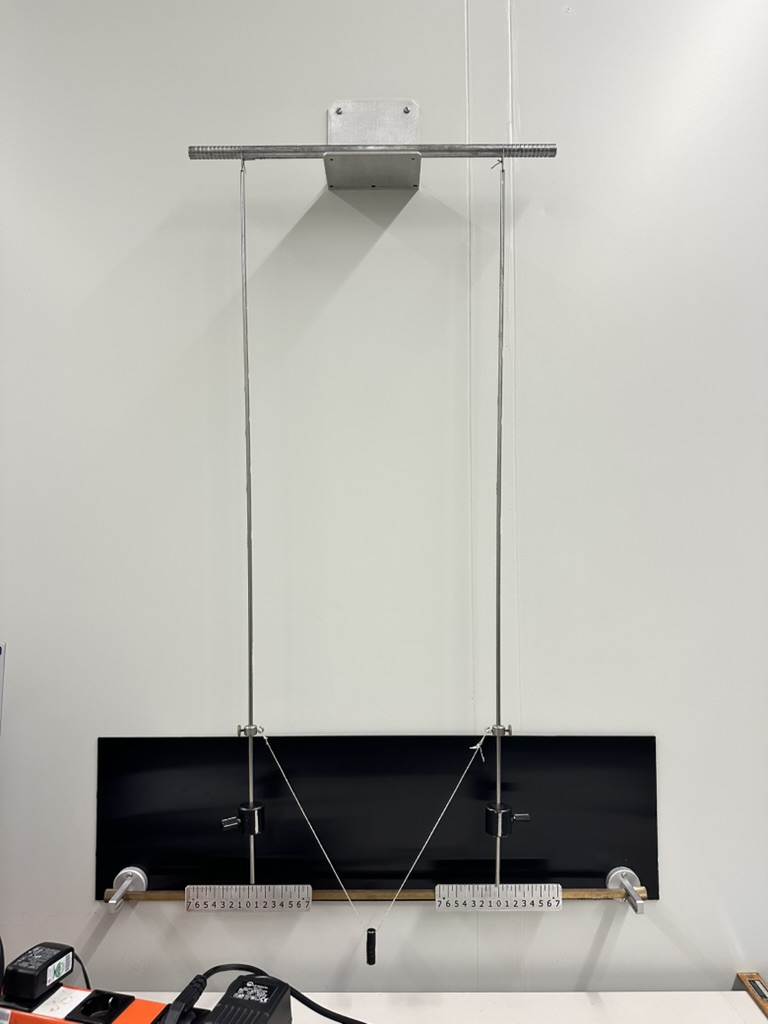
\includegraphics[width=0.4\textwidth]{Aufbau}}
%	\caption{Aufbau der Pendel, die hier bei \(\lh = \qty{70}{\centi\meter}\) gekoppelt sind.}
%	\label{fig:aufbau}
%\end{figure}

\section{Messwerte}

\begin{table}[H]
	\centering % damit die Tabelle trotzdem mittig steht
	\caption{Gemessene Spannung und Strom der Germanium-Diode.\label{tbl:GeDiode}}
	\begin{tabular}{ll}
		\toprule
		Spannung in \si{\milli\volt} & Strom in \si{\micro\ampere} \\
		\midrule
		\num{22,7}  & \num{0,06}  \\
		\num{100,2} & \num{11,9}  \\
		\num{152,0} & \num{55,5}  \\
		\num{199,3} & \num{182,3} \\
		\num{210,2} & \num{234,4} \\
		\num{220,2} & \num{292,3} \\
		\num{230,1} & \num{360}   \\
		\num{250,6} & \num{550}   \\
		\num{270,3} & \num{810}   \\
		\num{283,6} & \num{1050}  \\
		\num{320,3} & \num{1980}  \\
		\num{346,0} & \num{2990}  \\
		\num{366,0} & \num{4020}  \\
		\num{383,0} & \num{5020}  \\
		\num{397,0} & \num{5990}  \\
		\num{410,0} & \num{6990}  \\
		\num{422,0} & \num{8000}  \\
		\bottomrule
	\end{tabular}
\end{table}

\begin{table}[H]
	\centering % damit die Tabelle trotzdem mittig steht
	\caption{Gemessene Spannung und Strom der Silizium-Diode.\label{tbl:SiDiode}}
	\begin{tabular}{ll}
		\toprule
		Spannung in \si{\milli\volt} & Strom in \si{\micro\ampere} \\
		\midrule
		\num{99,4}  & \num{0,2} \\
		\num{155,2}  & \num{0,2} \\
		\num{208,2}  & \num{0,1} \\
		\num{304,6}  & \num{1}  \\
		\num{400}  & \num{11,8}  \\
		\num{452}  & \num{47,3}  \\
		\num{500}  & \num{149,3} \\
		\num{520}  & \num{238,9} \\
		\num{539}  & \num{355} \\
		\num{580}  & \num{820} \\
		\num{598}  & \num{1220} \\
		\num{623}  & \num{2020} \\
		\num{641}  & \num{2970} \\
		\num{655}  & \num{3980} \\
		\num{666}  & \num{5050} \\
		\num{674}  & \num{6020} \\
		\num{681}  & \num{7020} \\
		\num{687}  & \num{8010} \\
		\bottomrule
	\end{tabular}
\end{table}

\begin{table}[H]
	\centering % damit die Tabelle trotzdem mittig steht
	\caption{Gemessene Spannung und Strom der Silizium-Diode.\label{tbl:TempSi}}
	\begin{tabular}{lrr}
		\toprule
		Temperatur & Spannung in \si{\milli\volt} & Strom in \si{\micro\volt} \\
		\midrule
		\enquote{kalt} & \num{517} & \num{199,6} \\
		\enquote{warm} & \num{510} & \num{204,6}\\
		\bottomrule
	\end{tabular}
\end{table}

\begin{table}[H]
	\centering % damit die Tabelle trotzdem mittig steht
	\caption{Gemessene Spannung und Strom der Silizium-Diode.\label{tbl:TempGe}}
	\begin{tabular}{lrr}
		\toprule
		Temperatur & Spannung in \si{\milli\volt} & Strom in \si{\micro\volt} \\
		\midrule
		\enquote{kalt} & \num{201,9} & \num{200,4} \\
		\enquote{warm} & \num{191,5} & \num{207,4} \\
		\bottomrule
	\end{tabular}
\end{table}

\begin{table}[H]
	\centering % damit die Tabelle trotzdem mittig steht
	\caption{Gemessene Spannung und Strom der Silizium-Diode.\label{tbl:SiSperr}}
	\begin{tabular}{ll}
		\toprule
		Spannung in \si{\milli\volt} & Strom in \si{\micro\volt} \\
		\midrule
		\num{0,517} & \num{0,2} \\
		\num{1,061} & \num{0,3} \\
		\num{2,032} & \num{0,4} \\
		\num{3,220} & \num{0,5} \\
		\num{4,060} & \num{0,6} \\
		\num{5,120} & \num{0,7} \\
		\num{6,070} & \num{0,8} \\
		\num{7,060} & \num{0,9} \\
		\num{7,770} & \num{1,0} \\
		\bottomrule
	\end{tabular}
\end{table}

\begin{table}[H]
	\centering % damit die Tabelle trotzdem mittig steht
	\caption{Gemessene Spannung und Strom der Germanium-Diode.\label{tbl:GeSperr}}
	\begin{tabular}{ll}
		\toprule
		Spannung in \si{\milli\volt} & Strom in \si{\micro\volt} \\
		\midrule
		\num{0,518} & \num{0,7} \\
		\num{1,014} & \num{0,8} \\
		\num{1,527} & \num{0,9} \\
		\num{2,996} & \num{1,1} \\
		\num{4,050} & \num{1,2} \\
		\num{5,200} & \num{1,4} \\
		\num{6,000} & \num{1,5} \\
		\num{6,810} & \num{1,6} \\
		\num{7,510} & \num{1,7} \\
		\num{7,770} & \num{1,0} \\
		\bottomrule
	\end{tabular}
\end{table}




\section{Auswertung}


%\begin{figure}[H]
%	\centering{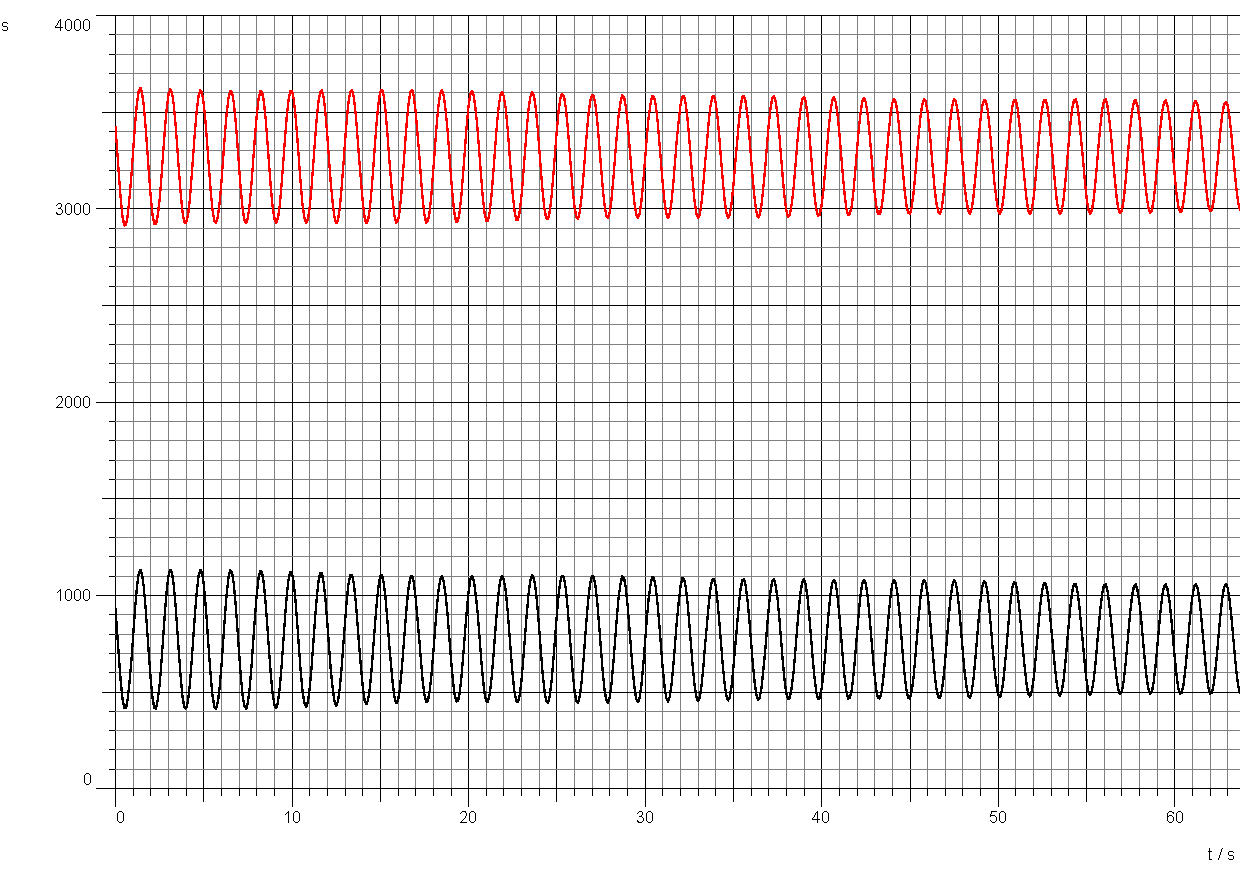
\includegraphics[width=0.7\textwidth]{gleichsinnige_FUNDAMENTALSCHWINGUNG_70cm.pdf}}
%	\caption{\(s(t)\)-Diagramm der gleichsinnigen Fundamentalschwingung bei \(\lh = \qty{70}{\centi\meter}\).}
%	\label{fig:gl70}
%\end{figure}

%\section{Fehlerrechnung}


\section{Zusammenfassung}

\begin{thebibliography}{999}
	\bibitem{Quelle} Versuchsanleitung zu \emph{M23 -- Gekoppelte Pendel} (Abgerufen am 25.09.2025).
	Online verfügbar unter: \url{https://www3.physik.uni-stuttgart.de/studium/praktika/ap/pdf_dateien/M23.pdf}
\end{thebibliography}

%\printbibliography
\section{Anhang}

%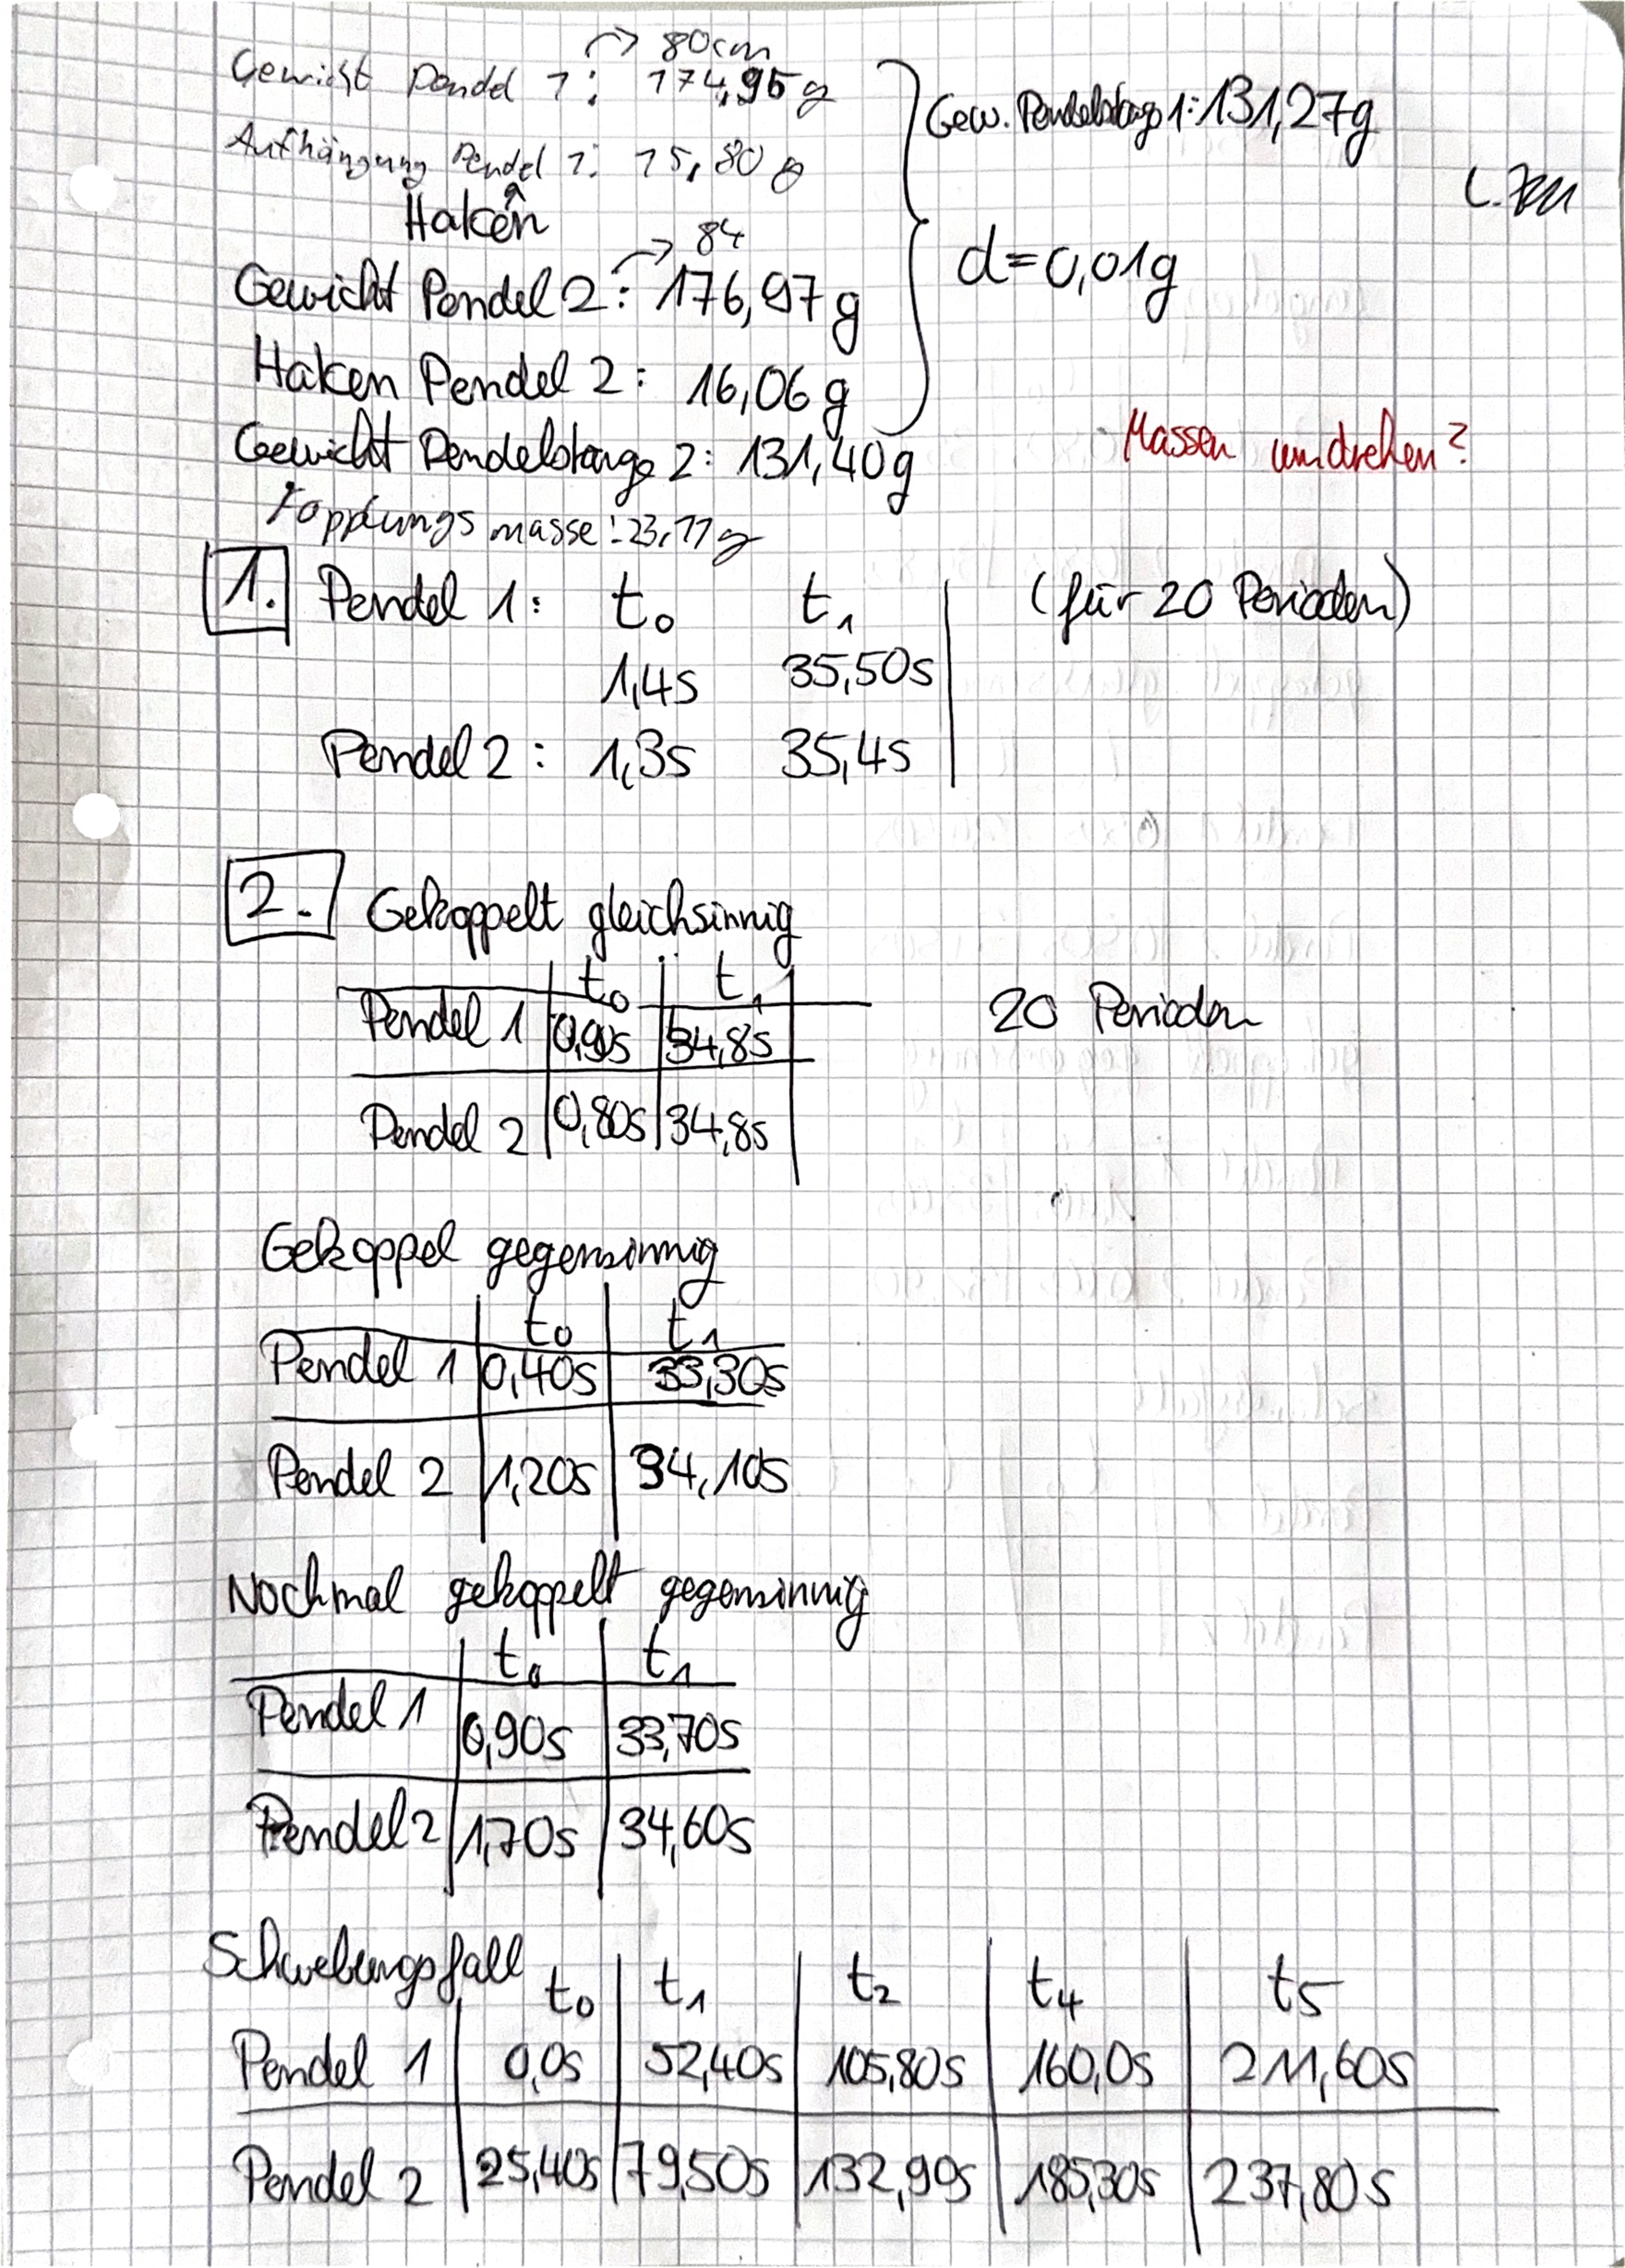
\includepdf[pages=-]{Messprotokoll.pdf}

\end{document}